\documentclass[a4paper]{article}
\usepackage[pdftex]{graphicx}
\usepackage[utf8]{inputenc}
\usepackage{enumerate}
\usepackage{siunitx}
\sisetup{locale=DE}
\usepackage{icomma}
\usepackage{amssymb}
\usepackage{tikz}
\usepackage{href-ul}
\hypersetup{
	colorlinks=true,
	linkcolor=blue,
	urlcolor=blue}
\usepackage{geometry}
\geometry{a4paper, top=15mm, left=15mm, right=15mm, bottom=15mm,
	headsep=10mm, footskip=12mm}

\begin{document}
	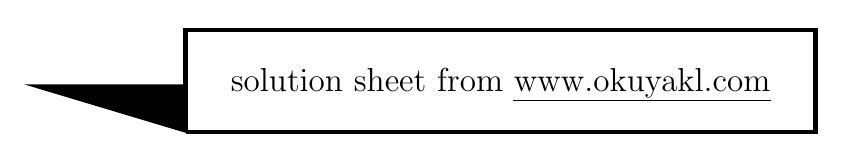
\begin{tikzpicture}(10,3)
		\draw[ultra thick](2,0) --(10,0) -- (10,1.3) --(2,1.3) -- (2,0);
		\draw[fill=black](2,0)-- (0,.6) -- (2,.6) -- (2,0);
		\node at (6,.6) {\large solution sheet from \href{http://www.okuyakl.com}{www.okuyakl.com}};
	\end{tikzpicture}
	\vspace{0.5 cm}
	
	\noindent{\bf Task 1. a)}\\
	The braking acceleration is:
	$$a= {\Delta v \over \Delta t} ={{108 \over 3.6}~\SI{}{\meter\over \second}\over \SI{0.04}{\second} }=\SI{750}{\meter\over {\second^2}} $$
	\vspace{0.5 cm}
	
	\noindent{\bf Task 1. b)}\\
	The braking force would then be:
	$$ F = m \cdot a = \SI{0.42}{\kilogram} \cdot \SI{750}{\meter\over {\second^2}}=\SI{315}{\newton}$$
	\vspace{0.5 cm}
	
	\noindent{\bf Task 2. a)}\\
	\begin{itemize}
		\item Phase 1: The body moves at a constant speed.
		\item Phase 2: It is braked to a standstill.
		\item Phase 3: Acceleration
		\item Phase 4: uniform movement
		\item Phase 5: Deceleration to a standstill
	\end{itemize}
	\vspace{0.5 cm}
	
	\noindent{\bf Task 2. b)}\\
	The path is the area under the curve. One square corresponds to $4~FE=\SI{4}{\meter}$ We count 8~m under the section in phase 1, 4~m under that in phase 2.
	\vspace{0.5 cm}
	
	\noindent{\bf Task 2. c)}\\
	In total there are 12.5 squares under the lines, i.e. 50~m.
	The average speed is:
	$$\bar v={\SI{50}{\meter} \over \SI{12}{\second}}=\SI{4,2}{\meter\over \second}$$
	\vspace{0.5 cm}
	
	\noindent{\bf Task 2. d)}\\
	Forces only occur in the acceleration and braking phases:
	\begin{itemize}
		\item Phase 2: $$ F = m \cdot {\Delta v \over \Delta t} = \SI{0.75}{\kilogram} \cdot {\SI{-4.0}{\meter\over \second} \over \SI{2}{\second}}=\SI{-1.5}{\newton}$$
		\item Phase 3: $$ F = \SI{0.75}{\kilogram} \cdot {\SI{6.0}{\meter\over \second} \over \SI{2}{\second}} =\SI{2,3}{\newton}$$
		\item Phase 5: $$ F = \SI{0.75}{\kilogram} \cdot {\SI{-6.0}{\meter\over \second} \over \SI{4}{\second} }=\SI{-1,1}{\newton}$$
	\end{itemize}
	In terms of magnitude, the force is greatest in phase 3.
	\vspace{0.5 cm}
	
	\noindent
	\begin{minipage}{0.6\textwidth}
		\noindent{\bf Task 2. e)}\\
		The formula for the relationship between distance and acceleration is:
		$$
		\renewcommand{\arraystretch}{2}
		\begin{array}{rcll}
			v^2 &=& 2 \cdot a \cdot s & |\sqrt{\quad}\\
			v &=& \sqrt{ 2 \cdot a \cdot s}\\
			v &=& \sqrt{{2\cdot \SI{4,0}{\meter\over {\second^2}}}\cdot \SI{32}{\meter}}&=\SI{16} {\meter\over \second}
		\end{array}
		$$
		The acceleration time is:
		$$ t = {v \over a} = {\SI{16}{\meter\over \second} \over \SI{4,0}{\meter\over {\second^2}}}= \SI {4,0}{\second}$$
		The body now has to travel 18~m; for this he needs:
		$$ t = {s \over v} = {\SI{18}{\meter} \over \SI{16}{\meter\over \second}}=\SI{1,1}{\second}$$
		So in total it needs 5.1~s.
	\end{minipage}
	\hfill
	\begin{minipage}{0.4\textwidth}
		\setlength{\unitlength}{1 cm}
		\begin{picture}(6,4)
			\put(0.5,0.5){\vector(1,0){5.5}}
			\put(0.5,0.5){\vector(0,1){4}}
			\put(0.5,0){0}
			\put(4.2,0.7){Time in s}
			\put(0.7,3.5){v in $\SI{}{\meter\over \second}$}
			\put(0.5,0.5){\line(1,1){2.5}}
			\put(3,3){\line(1,0){1.5}}
		\end{picture}
	\end{minipage}
	\vspace{0.5 cm}
	
	\noindent{\bf Task 3. a)}\\
	$$v = { s \over t} = {\SI{5000}{\meter} \over \SI{150}{\second}}=\SI{33,3}{\meter\over \second}$$
	$$v = 33.3 \cdot 3.6 = \SI{120}{\kilo\meter\over \hour}$$
	\vspace{0.5 cm}
	
	\noindent{\bf Task 3. b)}\\
	$$ t = {s \over v} = {\SI{5400}{\meter}\over \SI{33,3}{\meter\over \second}}= \SI{162}{\second} = \SI{2}{\minute}~\SI{42}{\second}$$
	\vspace{0.5 cm}
	
	\noindent{\bf Task 3. c)}\\
	$$ s = v \cdot t = \SI{125}{\kilo\meter\over \hour} \cdot \SI{1,6}{\hour} = \SI{200}{\kilo\meter}$$
	\vspace{0.5 cm}
	
	\noindent{\bf Task 3. d)}\\
	Uniform movement; Movement without acceleration.
	\vspace{0.5 cm}
	
	\noindent {\bf Exercise 4. a)}
	The acceleration a is ($v=\SI{55,6}{\meter\over \second}$):
	$$ a = {\Delta v \over \Delta t} = {\SI{55,6}{\meter\over\second} \over \SI{10}{\second}}= \SI{5,6 }{\meter\over {\second^2}}$$
	\vspace{0.5 cm}
	
	\noindent {\bf Exercise 4. b)}
	The required route is:
	$$ s = {1 \over 2}a\cdot t^2={1 \over 2}\cdot\SI{5,6}{\meter\over {\second^2}} \cdot (\SI{ 10}{\second})^2 = \SI{280}{\meter}$$
	\vspace{0.5 cm}
	
	\noindent {\bf Exercise 4. (i) and (ii)}
	Time-velocity diagram:
	\vspace{0.5 cm}
	
	\setlength{\unitlength}{1 cm}
	\begin{picture}(8,6)
		\put(0.5,0.5){\vector(1,0){7}}
		\put(0.5,0.5){\vector(0,1){5}}
		\put(0.5,0){0}
		\put(2.0,0){15}
		\put(5.0,0){45}
		\put(7,0){65}
		\put(7.2,0.7){Time in s}
		\put(0,3.5){60}
		\put(0,5){90}
		\put(0.7,5){v in $\SI{}{\meter\over\second}$}
		\put(0.5,0.5){\line(1,2){1.5}}
		\put(2,0.5){\line(0,1){3}}
		\put(2,3.5){\line(1,0){3}}
		\put(5,0.5){\line(0,1){3}}
		\put(5,3.5){\line(4,3){2}}
		\put(7,0.5){\line(0,1){4.5}}
		\put(1.5,1.5){$A_1$}
		\put(3.5,1.5){$A_2$}
		\put(5.5,1.5){$A_3$}
		\end{picture}
		\vspace{0.5 cm}
		
		\noindent We determine the areas under the curve (= distance traveled). $A_1$ is a triangle,
		$A_2$ is a rectangle and $A_3$ is a trapezoid.
		$$
		\begin{array}{ccc}
		A_1 =& 0.5 \cdot \SI{15}{\second} \cdot \SI{60}{\meter\over \second} &= \SI{450}{\meter}\\
		A_2 =& \SI{30}{\second} \cdot \SI{60}{\meter\over \second} &= \SI{1800}{\meter}\\
		A_3 =& 0.5 \cdot \SI{20}{\second} \cdot (60+90) \SI{}{\meter\over \second} &=\SI{1500}{\meter} \\
		& \textnormal{total} \, s=& \SI{3750}{\meter}
		\end{array}
		$$
		\begin{center}
		\includegraphics[width=7 cm]{../../viecher/eendcomic.pdf}
		
		Here you can go back to the \href{https://www.okuyakl.de/phys/p10kinL410/ae410.pdf}{task sheet}
		\end{center}
		
	\end{document}